\begin{center}
  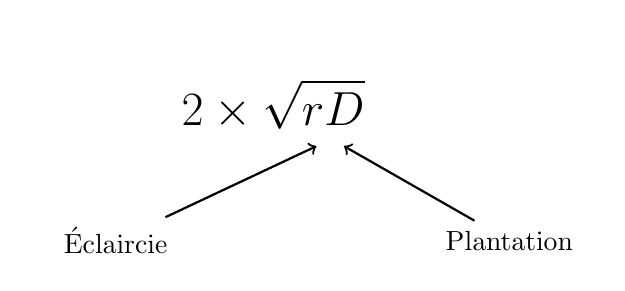
\begin{tikzpicture}[thick,every text node part/.style={align=center}]

    % --------------------------------------------------------- %
    % ------------- principal node (Formula)
    % --------------------------------------------------------- %
    \node[text width=6cm,minimum height=1cm,minimum width=3cm] (formule) at (10,10) {\LARGE{$$2 \times \sqrt{rD}$$}};

    % --------------------------------------------------------- %
    % ------------ Effect of forst management
    % --------------------------------------------------------- %
    \node[text width=2cm] (ecl) at (8,8) {Éclaircie};
    \draw[->]	(ecl) to node [midway] (formule) {} (10.55,9.2);

    \node[text width=2cm] (plant) at (13,8) {Plantation};
    \draw [->] (plant) to node [midway] (formule) {} (10.9,9.2);

  \end{tikzpicture}
\end{center}
